\documentclass{article}
\usepackage[T1]{fontenc}
\usepackage[utf8]{inputenc}
\usepackage{polski}
\usepackage{amsmath}
\usepackage{amssymb}
\usepackage{geometry}
\usepackage{graphicx}

\title{Projekt systemu autoryzacji w oparciu o funkcjonalność tokenów}

\geometry{
 a4paper,
 total={170mm,257mm},
 left=20mm,
 top=20mm,
}

\begin{document}

\maketitle

\clearpage

\tableofcontents

\clearpage

\section{Wstęp}

Wraz z dynamicznym rozwojem aplikacji internetowych oraz popularyzacją architektury rozproszonej, mechanizmy uwierzytelniania i autoryzacji stały się jednym z najbardziej krytycznych elementów systemów informatycznych. Zapewnienie bezpieczeństwa danych, przy jednoczesnym zachowaniu wysokiej wydajności i skalowalności, stanowi wyzwanie, z którym inżynierowie oprogramowania mierzą się od początków istnienia sieci WWW (ang. \textit{World Wide Web}).

\subsection{Rys historyczny i ewolucja mechanizmów uwierzytelniania}

We wczesnych fazach rozwoju aplikacji internetowych, serwery WWW generowały statyczne strony HTML, a potrzeba śledzenia tożsamości użytkownika była marginalna. Wraz z pojawieniem się dynamicznych serwisów i portali transakcyjnych, konieczne stało się wdrożenie mechanizmów pozwalających na zapamiętywanie stanu pomiędzy kolejnymi żądaniami klienta. 

Początkowo standardem stało się podejście oparte na sesjach (ang. \textit{Session-based Authentication}). W tym modelu po pomyślnym zalogowaniu użytkownika, serwer tworzył w swojej pamięci operacyjnej lub bazie danych obiekt sesji, a do przeglądarki klienta wysyłał jedynie unikalny identyfikator (tzw. \textit{Session ID}) zapisywany w pliku cookie. Przy każdym kolejnym żądaniu, przeglądarka automatycznie dołączała ciasteczko, a serwer weryfikował jego ważność, odpytując własną pamięć stanu. 

Rozwiązanie to, choć stosunkowo proste i bezpieczne, okazało się problematyczne w dobie nowoczesnych aplikacji internetowych (m.in. typu \textit{Single Page Application} - SPA) oraz architektur opartych na mikroserwisach. Utrzymywanie stanu na serwerze (ang. \textit{Stateful}) utrudniało skalowanie poziome (ang. \textit{Horizontal Scaling}) – jeśli żądanie użytkownika trafiło na inny węzeł serwera niż ten, na którym utworzono sesję, autoryzacja kończyła się niepowodzeniem, chyba że wdrożono skomplikowane mechanizmy replikacji sesji lub systemy centralnego buforowania (np. Redis).

\subsection{Protokół HTTP a bezstanowość}

Protokół HTTP (ang. \textit{Hypertext Transfer Protocol}), będący fundamentem komunikacji w sieci Web, z definicji jest protokołem bezstanowym (ang. \textit{Stateless}). Oznacza to, że każde żądanie wysyłane przez klienta do serwera jest traktowane jako całkowicie niezależna operacja. Serwer nie przechowuje żadnych informacji o poprzednich interakcjach z danym klientem na poziomie samego protokołu.

Bezstanowość HTTP jest jego ogromną zaletą, ponieważ pozwala na szybkie i wydajne obsługiwanie tysięcy jednoczesnych połączeń bez narzutu pamięciowego związanego z utrzymywaniem kontekstu. Z drugiej strony, wymusza to na twórcach oprogramowania implementację dodatkowych warstw logiki aplikacyjnej, które do każdego żądania dołączą dowód tożsamości użytkownika. Odpowiedzią na te architektoniczne i wydajnościowe wyzwania stało się uwierzytelnianie oparte na tokenach.

\subsection{Koncepcja autoryzacji opartej na tokenach}

W przeciwieństwie do autoryzacji sesyjnej, podejście oparte na tokenach (ang. \textit{Token-based Authentication}) realizuje postulat całkowitej bezstanowości (ang. \textit{Statelessness}) po stronie serwera. W tym modelu, po weryfikacji poświadczeń (np. loginu i hasła), serwer kryptograficznie podpisuje pakiet danych reprezentujący tożsamość i uprawnienia użytkownika, a następnie odsyła go do klienta w formie tokenu.

Od tego momentu klient przechowuje token (np. w pamięci lokalnej przeglądarki) i dołącza go do każdego żądania HTTP, zazwyczaj w nagłówku \texttt{Authorization} ze schematem \texttt{Bearer}. Serwer odbierający żądanie nie musi odpytywać bazy danych w celu weryfikacji sesji – wystarczy, że za pomocą swojego klucza prywatnego lub symetrycznego sprawdzi ważność podpisu kryptograficznego umieszczonego na tokenie. 

Podejście to idealnie wpisuje się w architekturę REST API, umożliwia łatwe skalowanie aplikacji oraz ułatwia integrację systemów zewnętrznych. Najpopularniejszym obecnie standardem w tej dziedzinie jest JWT (ang. \textit{JSON Web Token}), jednak nie jest on pozbawiony wad – przede wszystkim charakteryzuje się znacznym rozmiarem, co w przypadku dołączania do każdego żądania HTTP może generować niepotrzebny narzut sieciowy.

\subsection{Anatomia standardu JSON Web Token (JWT)}

Aby w pełni zrozumieć motywację stojącą za zaprojektowaniem autorskiego formatu tokenu, należy przeanalizować strukturę obecnie panującego standardu JWT (zdefiniowanego w dokumencie RFC 7519). Standardowy token JWT składa się z trzech części oddzielonych kropkami:

\begin{enumerate}
    \item \textbf{Nagłówek (Header):} Zawiera metadane opisujące typ tokenu oraz użyty algorytm kryptograficzny (np. HS256, RS256). Często przyjmuje postać JSON: \texttt{\{"alg":"HS256","typ":"JWT"\}}.
    \item \textbf{Ładunek (Payload):} Zawiera właściwe oświadczenia (ang. \textit{claims}), takie jak identyfikator użytkownika, czas wygaśnięcia, czy lista ról.
    \item \textbf{Podpis (Signature):} Zapewnia integralność danych, wyliczany na podstawie zakodowanego nagłówka, ładunku oraz klucza tajnego.
\end{enumerate}

Krytyczna analiza tego standardu uwidacznia jego redundancję w środowiskach zamkniętych. W architekturach, gdzie serwer autoryzacyjny i serwer zasobów to ta sama aplikacja (lub zestaw zaufanych mikroserwisów), przesyłanie w każdym żądaniu nagłówka informującego o typie algorytmu jest zbędne, ponieważ serwer posiada tę wiedzę ze swojej wewnętrznej konfiguracji. Usunięcie tego elementu oraz optymalizacja samego ładunku stanowią fundament optymalizacji sieciowej zaproponowanej w niniejszej pracy.

\subsection{Cel pracy}

Głównym celem niniejszej pracy jest zaprojektowanie oraz implementacja autorskiego, wysoce zoptymalizowanego systemu autoryzacji i uwierzytelniania w środowisku .NET, opartego o funkcjonalność tokenów. Zaproponowane rozwiązanie, będące autonomiczną biblioteką, stanowi alternatywę dla standardu JWT. 

Kluczowym założeniem projektu jest optymalizacja wydajnościowa i redukcja rozmiaru przesyłanych danych poprzez eliminację nagłówka tokenu oraz zastosowanie innowacyjnego, bitowego mechanizmu mapowania ról użytkowników za pomocą ciągów w formacie szesnastkowym (Hex). System został zaprojektowany z myślą o maksymalnej łatwości integracji z istniejącymi projektami opartymi o framework ASP.NET Core, oferując elastyczną abstrakcję warstwy danych i możliwość dynamicznego wstrzykiwania informacji bezpośrednio do tokenu.

\subsection{Skład pracy}

Niniejsza praca inżynierska została podzielona na logiczne części, które prowadzą czytelnika od założeń koncepcyjnych, poprzez architekturę, aż po szczegóły implementacyjne i przykłady użycia. Układ pracy przedstawia się następująco:

\begin{itemize}
    \item \textbf{Rozdział 1: Wstęp} – Wprowadza w domenę problemu, nakreśla rys historyczny mechanizmów autoryzacji oraz definiuje główny cel i zakres pracy.
    \item \textbf{Rozdział 2: Projekt i architektura systemu} – Omawia stos technologiczny, przewagi zaproponowanego rozwiązania nad istniejącymi standardami oraz przedstawia architekturę oprogramowania z wykorzystaniem diagramów UML (diagram klas, przypadków użycia oraz sekwencji).
    \item \textbf{Rozdział 3: Modele danych i algorytmy uwierzytelniania} – Koncentruje się na schemacie bazy danych, innowacyjnym mechanizmie kodowania ról za pomocą masek bitowych oraz warstwie kryptograficznej odpowiedzialnej za integralność tokenów.
    \item \textbf{Rozdział 4: Logika biznesowa i potok autoryzacji} – Opisuje szczegóły implementacyjne serwisów zarządzających tożsamością, mechanizm automatycznej synchronizacji ról (\textit{RoleBootstrapper}) oraz implementację filtrów autoryzacyjnych w potoku żądań HTTP.
    \item \textbf{Rozdział 5: Integracja i zastosowanie praktyczne} – Prezentuje sposób podłączenia stworzonej biblioteki do aplikacji testowej, jej konfigurację oraz przykłady zabezpieczania punktów końcowych API.
    \item \textbf{Rozdział 6: Podsumowanie} – Zbiera najważniejsze wnioski płynące z realizacji projektu oraz nakreśla możliwe kierunki dalszego rozwoju systemu.
\end{itemize}

\clearpage

\section{Projekt i architektura systemu autoryzacji}

Omawiane rozwiązanie zostało zaprojektowane jako modułowa biblioteka typu \textit{Class Library} (.csproj), której głównym celem jest dostarczenie mechanizmu uwierzytelniania i autoryzacji dla aplikacji opartych o protokół HTTP. System charakteryzuje się architekturą pozwalającą na łatwą integrację z istniejącymi projektami poprzez wstrzykiwanie zależności oraz wykorzystanie atrybutów dekorujących punkty końcowe (ang. \textit{endpoints}).

\subsection{Koncepcja tokenu autoryzacyjnego}

W przeciwieństwie do standardu JWT (JSON Web Token), zaprojektowany system wykorzystuje uproszczoną strukturę tokenu, zoptymalizowaną pod kątem specyficznych wymagań projektu. Token $T$ jest ciągiem znaków składającym się z dwóch segmentów oddzielonych separatorem kropki. Każdy z segmentów jest zakodowany przy użyciu algorytmu Base64.

Strukturę tokenu można zapisać wzorem:

$$ T = \text{Base64}(B) + \text{"."} + \text{Base64}(S) $$

gdzie:
\begin{itemize}
    \item $B$ - Ciało tokenu (Body), zawierające zserializowane dane użytkownika i metadane sesji.
    \item $S$ - Suma kontrolna (Checksum), gwarantująca integralność danych.
\end{itemize}

Model danych zawarty w ciele tokenu ($B$) zdefiniowano następująco:

\begin{verbatim}
public sealed class Token
{
    public Guid Id { get; set; }
    public Guid UserId { get; set; }
    public object Data { get; set; }
    public string UserRoles { get; set; }
    public DateTime ExpirationDate { get; set; }
}
\end{verbatim}

Zarówno tokeny dostępowe (ang. \textit{Access Tokens}), jak i tokeny odświeżające (ang. \textit{Refresh Tokens}) są przekazywane w nagłówkach zapytań HTTP, co zapewnia separację danych autoryzacyjnych od ciała żądania.

\subsection{Warstwa danych i abstrakcja bazy}

System został zaprojektowany z myślą o niezależności od konkretnego silnika bazodanowego. Domyślna implementacja wykorzystuje \textit{Entity Framework Core} w połączeniu z Microsoft SQL Server, jednak architektura umożliwia:
\begin{enumerate}
    \item Nadpisanie konfiguracji dla innych silników (np. MySQL, PostgreSQL).
    \item Integrację z istniejącą bazą danych aplikacji nadrzędnej poprzez implementację odpowiednich interfejsów.
\end{enumerate}

Schemat bazy danych opiera się na czterech kluczowych encjach: użytkownikach, rolach, powiązaniach użytkowników z rolami oraz tokenach odświeżających.

\subsubsection{Definicje modeli encji}

Poniżej przedstawiono strukturę klas reprezentujących tabele w bazie danych. Modele te stanowią fundament warstwy persystencji.

\begin{verbatim}
public sealed class RefreshToken
{
    public Guid Id { get; set; }
    public Guid UserId { get; set; }
    public DateTime ExpirationDate { get; set; }
}

public sealed class Role
{
    public Guid Id { get; set; }
    public int RoleNumber { get; set; }
    public string RoleCode { get; set; }
}

public class User
{
    public Guid Id { get; set; }
    public string Username { get; set; }
    public string Email { get; set; }
    public string HashedPassword { get; set; }
}

public sealed class UserRole
{
    public Guid Id { get; set; }
    public Guid UserId { get; set; }
    public Guid RoleId { get; set; }
}
\end{verbatim}

Bezpieczeństwo danych wrażliwych zapewnione jest poprzez mechanizmy kryptograficzne. Hasła użytkowników ($HashedPassword$) oraz sumy kontrolne tokenów podlegają procesowi szyfrowania przed zapisem lub transmisją.

\clearpage

\section{Mechanizmy kryptograficzne i integralność danych}

Bezpieczeństwo systemu autoryzacji opiera się na zapewnieniu integralności i niezaprzeczalności emitowanych tokenów. W tym celu zaimplementowano serwis \texttt{HashingService}, realizujący logikę podpisu cyfrowego oraz kodowania danych.

\subsection{Algorytm podpisu cyfrowego}

Do generowania sumy kontrolnej (podpisu) wykorzystano algorytm HMAC (ang. \textit{Keyed-Hash Message Authentication Code}) w oparciu o funkcję skrótu SHA-256. Wybór ten podyktowany jest wysokim poziomem bezpieczeństwa oraz wydajnością tego rozwiązania w środowisku .NET.

Proces tworzenia tokenu $T$ można przedstawić jako funkcję odwzorowującą obiekt danych $D$ i klucz tajny $K$ na łańcuch znaków:

$$ P_{b64} = \text{Base64Url}(\text{JSON}(D)) $$
$$ \sigma = \text{Base64Url}(\text{HMAC}_{\text{SHA256}}(K, P_{b64})) $$
$$ T = P_{b64} + \text{"."} + \sigma $$

gdzie:
\begin{itemize}
    \item $P_{b64}$ – ładunek (payload) zakodowany w formacie Base64Url.
    \item $\sigma$ – wygenerowany podpis cyfrowy.
    \item $K$ – klucz symetryczny przechowywany w konfiguracji serwera, niedostępny dla klienta.
\end{itemize}

\subsection{Implementacja serwisu haszującego}

Klasa \texttt{HashingService}, implementująca interfejs \texttt{IHashingService}, jest odpowiedzialna za wszystkie operacje kryptograficzne związane z cyklem życia tokenu. Kluczowe dla implementacji było dostosowanie standardowego kodowania Base64 do wymogów przesyłania danych w protokole HTTP (tzw. Base64Url Encoding). Standardowe znaki \texttt{+} oraz \texttt{/} zostały zastąpione odpowiednio przez \texttt{-} i \texttt{\_}, a znaki dopełnienia \texttt{=} zostały usunięte.

Poniższy listing prezentuje kod źródłowy serwisu:

\begin{verbatim}
using AJT.Contracts;
using AJT.Entities;
using AJT.Models;
using AJT.Options;
using Microsoft.Extensions.Options;
using Newtonsoft.Json;
using System.Security.Cryptography;
using System.Text;

namespace AJT.Services
{
    internal sealed class HashingService : IHashingService
    {
        private readonly IOptions<AJTOptions> _options;

        public HashingService(IOptions<AJTOptions> options)
        {
            _options = options;
        }

        public string Hash(Token token)
        {
            var tokenJson = JsonConvert.SerializeObject(token);
            var tokenJson64 = Base64UrlEncode(Encoding.UTF8.GetBytes(tokenJson));
            var signature = CreateSignature(tokenJson64, _options.Value.Secret);
            return string.Join('.', tokenJson64, signature);
        }

        public string Hash(RefreshToken refreshToken)
        {
            var tokenJson = JsonConvert.SerializeObject(refreshToken);
            var tokenJson64 = Base64UrlEncode(Encoding.UTF8.GetBytes(tokenJson));
            var signature = CreateSignature(tokenJson64, _options.Value.Secret);
            return string.Join('.', tokenJson64, signature);
        }

        public bool VerifiyHash(string token)
        {
            var parts = token.Split('.');
            if (parts.Length != 2)
                return false;

            string unsignedToken = parts[0];
            string signature = parts[1];
            string expectedSignature = CreateSignature(unsignedToken, 
                                                       _options.Value.Secret);

            return signature == expectedSignature;
        }

        public string DecodePayload(string hashedToken)
        {
            var parts = hashedToken.Split('.');
            if (parts.Length != 2)
                throw new ArgumentException("Invalid AJT");

            var payload = parts[0];
            var bytes = Base64UrlDecode(payload);
            return Encoding.UTF8.GetString(bytes);
        }

        private static string CreateSignature(string unsignedToken, string secret)
        {
            var keyBytes = Encoding.UTF8.GetBytes(secret);
            var messageBytes = Encoding.UTF8.GetBytes(unsignedToken);

            using var hmac = new HMACSHA256(keyBytes);
            var hash = hmac.ComputeHash(messageBytes);
            return Base64UrlEncode(hash);
        }

        private static string Base64UrlEncode(byte[] input)
        {
            return Convert.ToBase64String(input)
                .TrimEnd('=')
                .Replace('+', '-')
                .Replace('/', '_');
        }

        private static byte[] Base64UrlDecode(string input)
        {
            string padded = input.Replace('-', '+').Replace('_', '/');
            switch (padded.Length % 4)
            {
                case 2: padded += "=="; break;
                case 3: padded += "="; break;
            }
            return Convert.FromBase64String(padded);
        }
    }
}
\end{verbatim}

\subsection{Weryfikacja tokenu}

Proces weryfikacji (\texttt{VerifiyHash}) nie polega na odszyfrowaniu podpisu, lecz na jego ponownym wyliczeniu. System pobiera część tokenu zawierającą dane, generuje dla niej podpis przy użyciu tego samego sekretnego klucza $K$, a następnie porównuje wynik z podpisem przesłanym przez klienta. Zgodność obu ciągów znaków potwierdza, że dane nie zostały zmodyfikowane w trakcie transmisji oraz że token został wygenerowany przez zaufane źródło.

\subsection{Diagram przypadków użycia}

Diagram przypadków użycia (ang. \textit{Use Case Diagram}) modeluje interakcje pomiędzy aktorami systemu a jego głównymi funkcjonalnościami. W zaprojektowanym rozwiązaniu zidentyfikowano trzech głównych aktorów, ułożonych w hierarchii dziedziczenia uprawnień:

\begin{enumerate}
    \item \textbf{Niezalogowany użytkownik (Gość):} Aktor ten ma najniższy poziom uprawnień. Jego interakcja z systemem ogranicza się do prób uwierzytelnienia (logowania) w celu uzyskania pary tokenów oraz do ewentualnej rejestracji nowego konta w bazie danych.
    \item \textbf{Zalogowany użytkownik:} Aktor posiadający ważny token dostępowy. Dziedziczy on możliwości gościa, a dodatkowo może odświeżać swoją sesję przy użyciu \textit{Refresh Tokenu} oraz odpytywać punkty końcowe zabezpieczone podstawowym atrybutem \texttt{[RequireAuthentication]}.
    \item \textbf{Administrator:} Zalogowany użytkownik posiadający przypisaną odpowiednią rolę (np. "admin"). Aktor ten ma dostęp do punktów końcowych z restrykcjami ról (atrybut \texttt{[AllowRole]}) oraz posiada uprawnienia do zarządzania systemem, m.in. dynamicznego nadawania i odbierania ról innym użytkownikom.
\end{enumerate}

\begin{figure}[h]
    \centering
    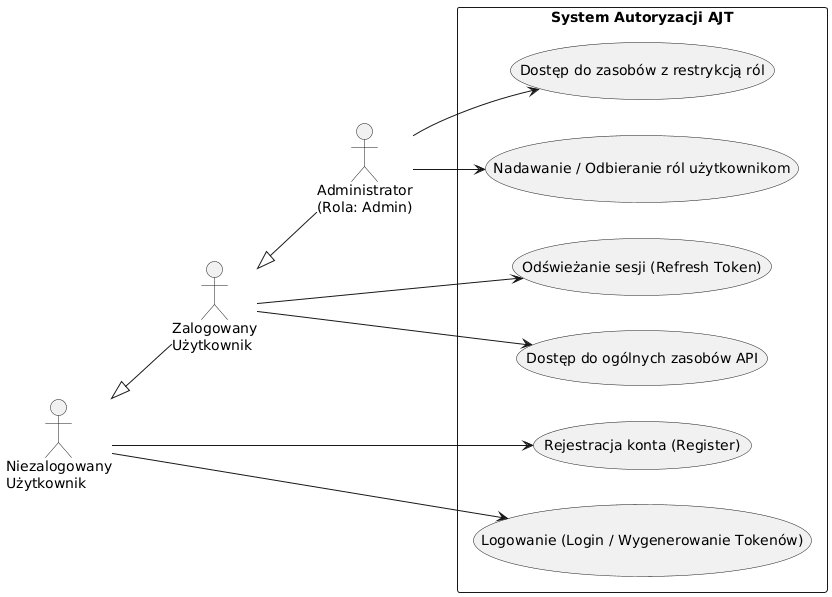
\includegraphics[width=0.8\textwidth]{png/usecase_diagram.png}
    \caption{Diagram przypadków użycia systemu autoryzacji}
    \label{fig:usecase_diagram}
\end{figure}

\clearpage

\subsection{Diagram sekwencji: Przepływ autoryzacji}

Diagram sekwencji (ang. \textit{Sequence Diagram}) szczegółowo obrazuje dynamiczny przepływ komunikatów pomiędzy obiektami systemu w czasie. Na potrzeby dokumentacji wybrano najbardziej złożony scenariusz: żądanie dostępu do punktu końcowego zabezpieczonego konkretną rolą (wykorzystanie filtru \texttt{AllowRoleFilter}).

Przepływ rozpoczyna się w momencie wysłania przez klienta HTTP żądania zawierającego nagłówek autoryzacyjny z tokenem \textit{Bearer}. Żądanie to jest przechwytywane przez mechanizm filtrów frameworka ASP.NET Core, zanim dotrze do właściwej logiki kontrolera. Następnie filtr oddelegowuje zadanie weryfikacji kryptograficznej do serwisu \texttt{HashingService}. Po potwierdzeniu integralności tokenu i odczytaniu jego ładunku (\textit{payload}), następuje deserializacja danych i weryfikacja daty ważności.

Kluczowym momentem ukazanym na diagramie jest wywołanie metody \texttt{DecodeRoles} z serwisu \texttt{RoleService}. Serwis ten pobiera definicje ról z bazy danych, a następnie wykonuje operacje bitowe na ciągu szesnastkowym odczytanym z tokenu, dekodując uprawnienia użytkownika. Wynikowa lista ról jest konfrontowana z wymaganiami punktu końcowego. W przypadku zgodności, filtr przepuszcza żądanie do kontrolera, który generuje odpowiedź \texttt{200 OK}. W przeciwnym razie potok zostaje przerwany, a klient otrzymuje status błędu (np. \texttt{401 Unauthorized} lub \texttt{403 Forbidden}).

\begin{figure}[h]
    \centering
    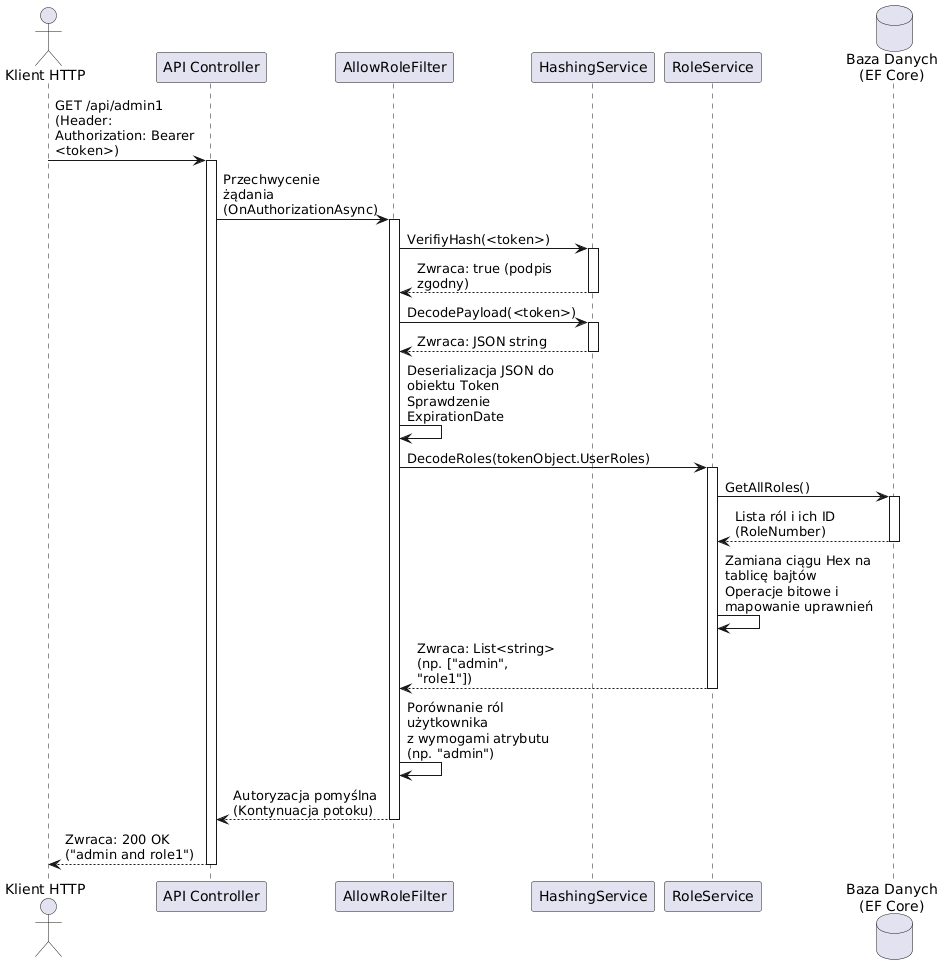
\includegraphics[width=1\textwidth]{png/sequence_diagram.png}
    \caption{Diagram sekwencji przedstawiający proces weryfikacji uprawnień}
    \label{fig:sequence_diagram}
\end{figure}

\clearpage

\subsection{Struktura implementacyjna i organizacja kodu}

Zaprojektowany system autoryzacji został zaimplementowany jako niezależna biblioteka klas (projekt typu \textit{Class Library} z rozszerzeniem \texttt{.csproj}). Architektura kodu źródłowego opiera się na ścisłym podziale obowiązków (ang. \textit{Separation of Concerns}), co ułatwia zarządzanie projektem, jego testowanie oraz ewentualną rozbudowę w przyszłości.

Kod został zorganizowany w logiczne przestrzenie nazw (ang. \textit{namespaces}), odzwierciedlające fizyczną strukturę katalogów w repozytorium projektu:

\begin{itemize}
    \item \textbf{AJT.Attributes} – warstwa dostępu i filtracji. Odpowiada za integrację z potokiem żądań HTTP frameworka ASP.NET Core. Znajdują się tu definicje atrybutów zabezpieczających (np. \texttt{AllowRole} oraz \texttt{RequireAuthentication}). Dodatkowo umieszczono tutaj filtry autoryzacyjne (m.in. \texttt{AllowRoleFilter}), które pełnią rolę pomostu między warstwą sieciową a logiką biznesową.
    
    \item \textbf{AJT.Contracts} – warstwa abstrakcji. Zgrupowano w niej wszystkie interfejsy systemu, w tym kontrakty serwisów (np. \texttt{ILoginService}, \texttt{IRoleService}) oraz interfejsy repozytoriów. Wydzielenie kontraktów do osobnego katalogu jest kluczowe dla poprawnego działania mechanizmu wstrzykiwania zależności (DI). Ułatwia to również tworzenie atrap (ang. \textit{mocks}) na potrzeby testów jednostkowych.
    
    \item \textbf{AJT.Entities} – warstwa persystencji danych. Zawiera modele (klasy C\#) bezpośrednio odwzorowujące tabele w relacyjnej bazie danych, wykorzystywane przez silnik Entity Framework Core (np. \texttt{User}, \texttt{Role}, \texttt{UserRole}).
    
    \item \textbf{AJT.Models} – obiekty transferu danych (DTO). Obejmuje struktury wykorzystywane do przenoszenia informacji pomiędzy warstwami aplikacji lub bezpośrednio do klienta, takie jak zdeserializowana forma tokenu (\texttt{Token}) czy obiekt zwracany po pomyślnym logowaniu (\texttt{CombinedToken}).
    
    \item \textbf{AJT.Options} – konfiguracja biblioteki. Zawiera klasy ułatwiające mapowanie ustawień podawanych podczas inicjalizacji systemu (np. \texttt{AJTOptions}), przechowujące m.in. klucze szyfrujące, czasy życia tokenów oraz tryby działania mechanizmu synchronizacji ról.
    
    \item \textbf{AJT.Services} – warstwa logiki biznesowej. Stanowi rdzeń całego systemu. Zgrupowano tu implementacje serwisów odpowiedzialnych za operacje kryptograficzne, autoryzację, zarządzanie uprawnieniami (w tym operacje na ciągach bitowych) oraz mechanizmy działające w tle (np. \texttt{RoleBootstrapper} implementujący interfejs \texttt{IHostedService}).
\end{itemize}

Wykorzystanie wzorca projektowego \textit{Fasada} oraz rozszerzeń kontenera wstrzykiwania zależności (implementacja metod \textit{Extension Methods} dla interfejsu \texttt{IServiceCollection}) sprawia, że cała wewnętrzna złożoność strukturalna biblioteki pozostaje ukryta przed programistą integrującym rozwiązanie. Z perspektywy aplikacji nadrzędnej, implementacja sprowadza się do wywołania pojedynczej metody konfiguracyjnej \texttt{UseAJT} podczas startu serwera.

\subsection{Zastosowanie wzorca wstrzykiwania zależności}

Architektura całego systemu została oparta na paradygmacie odwrócenia sterowania (ang. \textit{Inversion of Control} -- IoC) oraz wzorcu wstrzykiwania zależności (ang. \textit{Dependency Injection} -- DI). Zamiast bezpośrednio tworzyć instancje obiektów wewnątrz klas (co prowadzi do silnego sprzężenia kodu, ang. \textit{tight coupling}), komponenty systemu komunikują się ze sobą wyłącznie za pośrednictwem interfejsów abstrakcyjnych (warstwa \texttt{AJT.Contracts}).

Rozwiązanie to przynosi wymierne korzyści inżynierskie:
\begin{itemize}
    \item \textbf{Testowalność:} Możliwość łatwego wstrzyknięcia obiektów zastępczych (atrap) podczas pisania zautomatyzowanych testów jednostkowych.
    \item \textbf{Wymienialność komponentów:} Programista integrujący bibliotekę może w łatwy sposób podmienić domyślną implementację np. serwisu haszującego hasła, bez konieczności ingerencji w kod źródłowy samej biblioteki.
    \item \textbf{Zarządzanie cyklem życia:} Kontener DI dostarczany przez środowisko ASP.NET Core automatycznie zarządza pamięcią, tworząc i niszcząc instancje serwisów w zależności od ich skonfigurowanego cyklu życia (np. \textit{Scoped} dla operacji bazodanowych na pojedyncze żądanie HTTP, czy \textit{Singleton} dla bezstanowych serwisów kryptograficznych).
\end{itemize}

\clearpage

\subsection{Diagramy klas systemu}

Z uwagi na rozbudowaną architekturę biblioteki oraz zachowanie zasady pojedynczej odpowiedzialności (ang. \textit{Single Responsibility Principle}), struktura statyczna systemu została podzielona na trzy logiczne obszary. Zobrazowano je za pomocą oddzielnych diagramów klas, co pozwala na precyzyjne prześledzenie relacji w poszczególnych warstwach.

\subsubsection{Warstwa danych (Persystencja)}

Pierwszy diagram (Rysunek \ref{fig:class_entities}) prezentuje encje bazodanowe zgrupowane w przestrzeni nazw \texttt{AJT.Entities}. Relacje pomiędzy klasami odzwierciedlają strukturę tabel w relacyjnej bazie danych. Widoczne jest powiązanie użytkownika (\texttt{User}) z tokenami odświeżającymi (\texttt{RefreshToken}) relacją jeden-do-wielu, a także przypisanie użytkowników do ról (\texttt{Role}) poprzez tabelę łącznikową \texttt{UserRole}.

\begin{figure}[h]
    \centering
    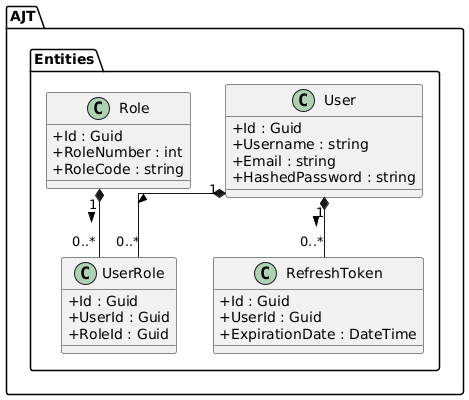
\includegraphics[width=0.7\textwidth]{png/class_entities.png}
    \caption{Diagram klas warstwy danych (Entities)}
    \label{fig:class_entities}
\end{figure}

\clearpage

\subsubsection{Warstwa kontraktów i modeli wymiany danych}

Drugi diagram (Rysunek \ref{fig:class_contracts}) skupia się na interfejsach definiujących możliwości systemu (\texttt{AJT.Contracts}) oraz modelach DTO (\texttt{AJT.Models}). Oddzielenie definicji (interfejsów) od ich implementacji jest fundamentem mechanizmu wstrzykiwania zależności (DI) wykorzystywanego w całym projekcie. Dodatkowo zaprezentowano strukturę samego tokenu oraz obiektu \texttt{CombinedToken}.

\begin{figure}[h]
    \centering
    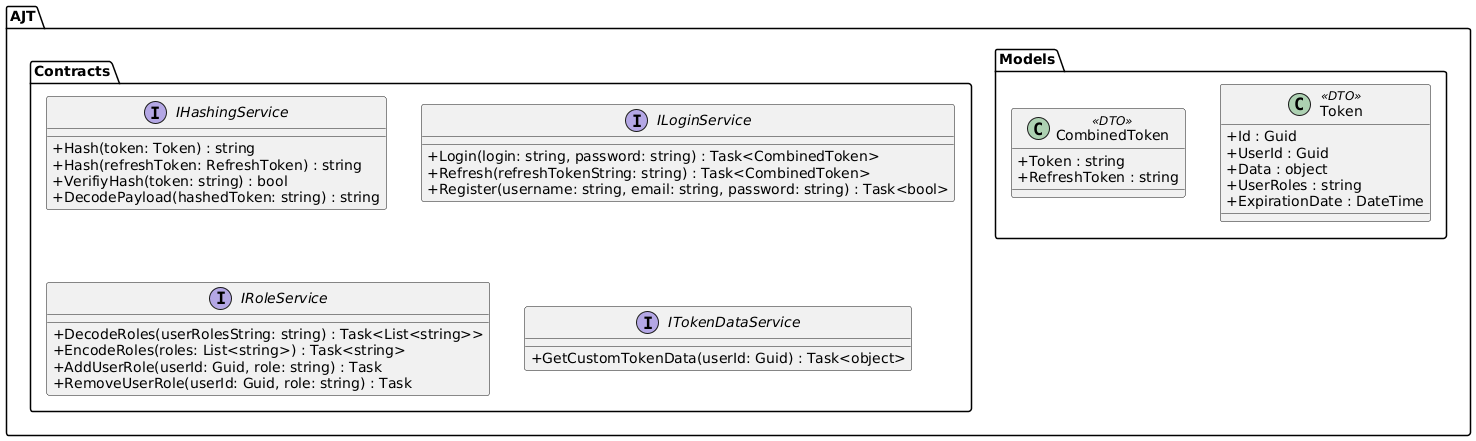
\includegraphics[width=0.8\textwidth]{png/class_contracts.png}
    \caption{Diagram klas warstwy kontraktów i modeli (DTO)}
    \label{fig:class_contracts}
\end{figure}

\subsubsection{Warstwa implementacji logiki i punktów dostępu}

Trzeci diagram (Rysunek \ref{fig:class_services}) obrazuje konkretne implementacje serwisów (\texttt{AJT.Services}) oraz filtry autoryzacyjne (\texttt{AJT.Attributes}). Strzałki zależności (przerywane) wyraźnie pokazują, w jaki sposób potok żądań HTTP (poprzez \texttt{AllowRoleFilter}) korzysta z wstrzykniętych serwisów do walidacji kryptograficznej oraz dekodowania ról bitowych.

\begin{figure}[h]
    \centering
    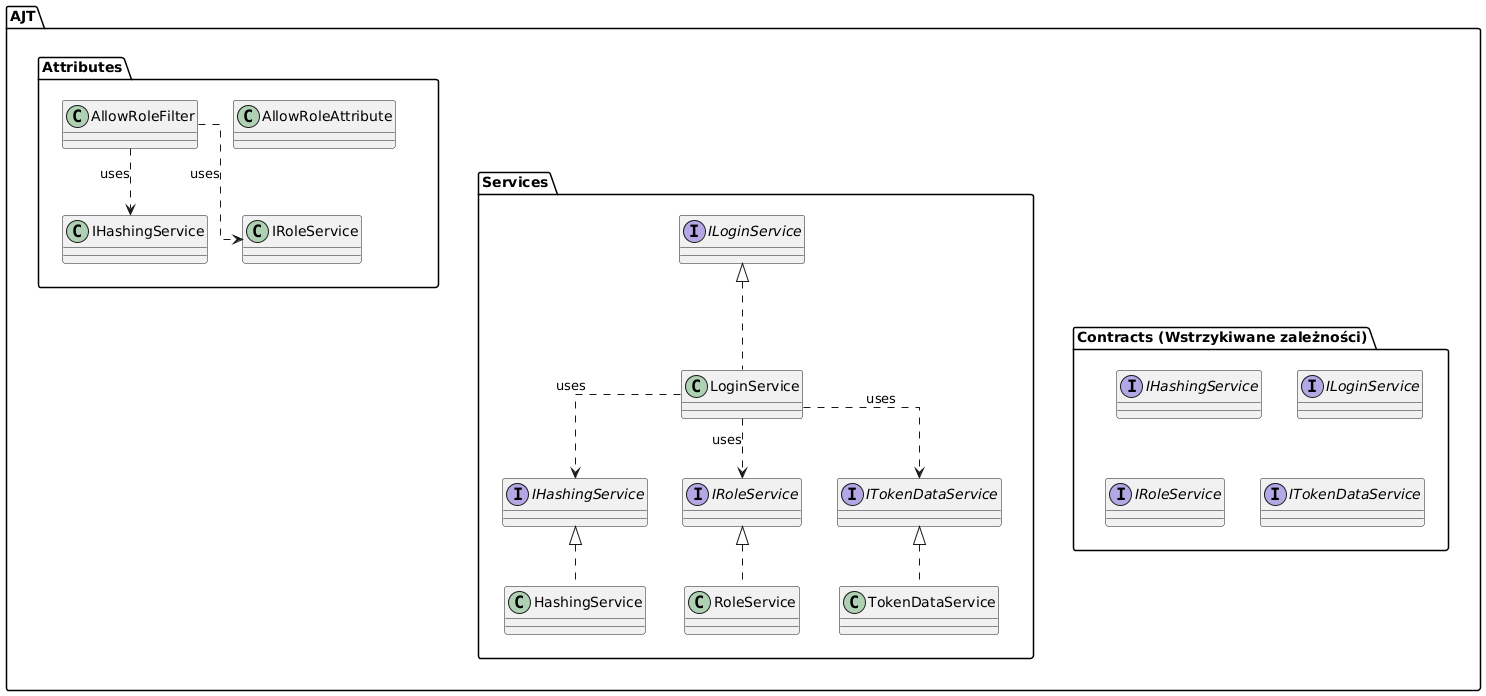
\includegraphics[width=0.85\textwidth]{png/class_services.png}
    \caption{Diagram klas implementacji logiki biznesowej i atrybutów}
    \label{fig:class_services}
\end{figure}

\clearpage

\subsection{Mechanizm zarządzania rolami}

Istotnym elementem systemu jest zoptymalizowany sposób przechowywania i weryfikacji uprawnień. Każda rola w systemie posiada unikalny identyfikator liczbowy $R_{id} \in \mathbb{N}$. Zbiór ról przypisanych do użytkownika nie jest przechowywany jako lista obiektów, lecz jako łańcuch znaków w formacie szesnastkowym (Hex), reprezentujący maskę bitową.

Mechanizm ten zakłada, że posiadanie roli o identyfikatorze $n$ odpowiada ustawieniu $n$-tego bitu w ciągu binarnym na wartość 1. Otrzymana liczba jest następnie konwertowana na system szesnastkowy. Aby zminimalizować narzut danych przesyłanych w tokenie, zastosowano zmienną długość ciągu wynikowego – długość łańcucha Hex jest zależna od najwyższego identyfikatora roli posiadanej przez użytkownika.

$$ UserRoles_{hex} = \text{Hex}(\sum_{i \in R_{user}} 2^i) $$

Taka konstrukcja pozwala na błyskawiczną weryfikację uprawnień poprzez operacje bitowe, bez konieczności iterowania po kolekcjach obiektów w trakcie przetwarzania każdego żądania HTTP.

\subsubsection{Przykład konwersji uprawnień na maskę bitową}

Aby lepiej zobrazować działanie algorytmu kompresji, warto prześledzić proces na konkretnym przypadku użycia. Załóżmy, że w systemie zdefiniowano słownik zawierający trzy podstawowe role:
\begin{itemize}
    \item $R_0$: "user" (Identyfikator: 0)
    \item $R_1$: "moderator" (Identyfikator: 1)
    \item $R_2$: "admin" (Identyfikator: 2)
\end{itemize}

Jeśli dany użytkownik posiada role "user" oraz "admin", system wylicza jego uprawnienia ustawiając bit zerowy oraz bit drugi na wartość 1. W reprezentacji binarnej (czytanej od prawej do lewej, gdzie najmniej znaczący bit znajduje się po prawej stronie), otrzymujemy ciąg:

$$ 00000101_2 $$

Zgodnie z systemem wag dwójkowych, wartość dziesiętna tego ciągu wynosi:

$$ 1 \cdot 2^2 + 0 \cdot 2^1 + 1 \cdot 2^0 = 4 + 0 + 1 = 5_{10} $$

W ostatnim kroku liczba dziesiętna konwertowana jest na format szesnastkowy (Hex). Liczba 5 w systemie szesnastkowym to po prostu \texttt{05}. Taki dwuznakowy ciąg jest dopisywany do tokenu. Kiedy użytkownik wysyła żądanie do punktu końcowego zabezpieczonego rolą "moderator" ($R_1$), system wykonuje operację iloczynu logicznego (AND) na masce bitowej żądania i masce wymaganej:

$$ 00000101_2 \text{ AND } 00000010_2 = 00000000_2 $$

Wynik równy zeru jednoznacznie informuje filtr autoryzacyjny, że użytkownik nie posiada wymaganego uprawnienia, co skutkuje odrzuceniem żądania w czasie rzędu $O(1)$.

\subsection{Algorytmika obsługi ról bitowych}

Kluczowym aspektem wydajnościowym systemu jest sposób reprezentacji ról. Zamiast przesyłać w tokenie pełne nazwy ról, system operuje na ciągu szesnastkowym (Hex), który jest reprezentacją tablicy bajtów.

Logika konwersji została zaimplementowana w serwisie \texttt{RoleService}. Metoda \texttt{DecodeRoles} przekształca ciąg Hex na tablicę bajtów, a następnie iteruje po poszczególnych bitach. Jeśli $j$-ty bit w $i$-tym bajcie jest ustawiony na 1, oznacza to, że użytkownik posiada rolę o numerze identyfikacyjnym obliczanym ze wzoru:

$$ ID_{roli} = i \cdot 8 + j $$

Analogicznie, proces kodowania (\texttt{EncodeRoles}) polega na mapowaniu kodów ról na ich numery, a następnie ustawianiu odpowiednich bitów w tablicy bajtów przy użyciu logicznej sumy (OR) oraz przesunięcia bitowego.

Poniższy fragment kodu prezentuje implementację metod kodujących i dekodujących role:

\begin{verbatim}
public async Task<List<string>> DecodeRoles(string userRolesString)
{
    using var scope = _scopeFactory.CreateScope();
    var roleRepo = scope.ServiceProvider.GetRequiredService<IRoleRepo>();
    var dbRoles = await roleRepo.GetAllRoles();
    
    int byteCount = userRolesString.Length / 2;
    byte[] bytes = new byte[byteCount];
    for (int i = 0; i < byteCount; i++)
        bytes[i] = Convert.ToByte(userRolesString.Substring(i * 2, 2), 16);

    var result = new List<string>();

    for (int byteIndex = 0; byteIndex < bytes.Length; byteIndex++)
    {
        for (int bit = 0; bit < 8; bit++)
        {
            int bitIndex = byteIndex * 8 + bit;
            bool isSet = (bytes[byteIndex] & (1 << bit)) != 0;
            if (isSet)
            {
                var role = dbRoles.FirstOrDefault(r => 
                    r.RoleNumber == bitIndex)?.RoleCode;
                if (role != null)
                    result.Add(role);
            }
        }
    }
    return result;
}

public async Task<string> EncodeRoles(List<string> roles)
{
    using var scope = _scopeFactory.CreateScope();
    var roleRepo = scope.ServiceProvider.GetRequiredService<IRoleRepo>();
    var dbRoles = await roleRepo.GetAllRoles();
    var userRoles = new Dictionary<int, string>();

    int maxBit = 0;
    foreach (var role in roles)
    {
        var roleNumber = dbRoles.FirstOrDefault(x => 
            x.RoleCode == role)?.RoleNumber ?? 0;
        userRoles.Add(roleNumber, role);
        if (maxBit < roleNumber)
            maxBit = roleNumber;
    }

    int byteCount = (maxBit / 8) + 1;
    byte[] bytes = new byte[byteCount];

    foreach (var kv in userRoles)
    {
        int bitIndex = kv.Key;
        int byteIndex = bitIndex / 8;
        int bitInByte = bitIndex % 8;
        bytes[byteIndex] |= (byte)(1 << bitInByte);
    }

    return BitConverter.ToString(bytes).Replace("-", "");
}
\end{verbatim}

Takie podejście pozwala na znaczną redukcję rozmiaru tokenu, co jest istotne w kontekście przesyłania danych w nagłówkach HTTP przy każdym zapytaniu.

\clearpage

\subsection{Logika biznesowa i potok autoryzacji}

Głównym elementem modułu, który odpowiada za zarządzanie tożsamością oraz integrację z frameworkiem ASP.NET Core, jest warstwa serwisów i filtrów. W tym rozdziale opisano proces generowania tokenów, automatyzację w zarządzaniu słownikami ról, a także mechanizm przechwytywania zapytań HTTP.
\subsection{Proces logowania i generowania tokenów}

Proces uwierzytelniania agreguje logikę rejestracji, logowania oraz odświeżania sesji. Za te operacje odpowiada \texttt{LoginService}. Kluczowym elementem jest metoda \texttt{CreateCombinedTokenForUser}, która orkiestruje budowę finalnego obiektu po poprawnej weryfikacji hasła:

\begin{enumerate}
    \item Pobranie ról użytkownika i ich kompresja do formatu Hex.
    \item Pobranie dodatkowych, niestandardowych danych zdefiniowanych przez programistę aplikacji nadrzędnej.
    \item Podpisanie obu tokenów (Access i Refresh) i zwrócenie ich do kontrolera.
\end{enumerate}

Poniższy listing przedstawia kluczowy fragment serwisu logowania:

\begin{verbatim}
public async Task<CombinedToken?> Login(string login, string password)
{
    var hashedPassword = _passwordHasher.HashPassword(password);

    using var scope = _scopeFactory.CreateScope();
    var userRepo = scope.ServiceProvider.GetRequiredService<IUserRepo>();
    var user = await userRepo.GetUserByLogin(login);

    if (user is null || user.HashedPassword != hashedPassword)
        return null;

    return await CreateCombinedTokenForUser(scope, user);
}

private async Task<CombinedToken?> CreateCombinedTokenForUser(
    IServiceScope scope, User user)
{
    var userRoleRepo = scope.ServiceProvider.GetRequiredService<IUserRoleRepo>();
    var roles = await userRoleRepo.GetUserRoles(user);

    var token = new Token
    {
        Id = Guid.NewGuid(),
        UserId = user.Id,
        Data = await _tokenDataService.GetCustomTokenData(user.Id),
        ExpirationDate = DateTime.Now.Add(_options.Value.TokenExpirationTime)
    };

    if (roles is not null)
        token.UserRoles = await _roleService.EncodeRoles(
            roles.Select(x => x.RoleCode).ToList());

    var refreshTokenRepo = scope.ServiceProvider
                                .GetRequiredService<IRefreshTokenRepo>();

    var refreshToken = new RefreshToken
    {
        UserId = user.Id,
        ExpirationDate = DateTime.Now.Add(
            _options.Value.RefreshTokenExpirationTime)
    };
    await refreshTokenRepo.AddRefreshToken(refreshToken);

    return new CombinedToken
    {
        Token = _hashingService.Hash(token),
        RefreshToken = _hashingService.Hash(refreshToken)
    };
}
\end{verbatim}

\subsection{Dynamiczne rozszerzanie ładunku tokenu}

Aby uniknąć sztywnego wiązania struktury tokenu z modelem biznesowym, zastosowano mechanizm delegatów. Klasa \texttt{TokenDataService} pełni rolę pośrednika, który umożliwia wstrzyknięcie dowolnego obiektu do pola \texttt{Data} w tokenie. 

Mechanizm ten opiera się na delegacie \texttt{Func}, który przyjmuje identyfikator użytkownika oraz dostawcę usług \texttt{IServiceProvider}. Dzięki temu, w momencie generowania tokenu programista może odpytać bazę danych o dowolne informacje domenowe (np. dział pracownika) i dołączyć je do payloadu.

\subsection{Automatyzacja zarządzania uprawnieniami (RoleBootstrapper)}

W celu zapewnienia spójności między kodem aplikacji a stanem bazy danych, system wyposażono w moduł automatycznej synchronizacji ról zaimplementowany jako \texttt{IHostedService}. 

W trybie automatycznym algorytm wykorzystuje mechanizm refleksji (\textit{System.Reflection}) do przeszukiwania klas oraz metod. Celem operacji jest odnalezienie wszystkich atrybutów autoryzacyjnych. Zebrane z kodu unikalne nazwy ról tworzą zbiór, który system następnie porównuje ze stanem bazy danych. Jeśli wykryte zostaną rozbieżności, podczas startu aplikacji następuje przebudowa tabeli ról. Zapewnia to przypisanie każdej roli unikalnego numeru ID, co jest niezbędne do poprawnego działania mechanizmu masek bitowych.
\subsection{Implementacja potoku autoryzacji HTTP}

Dostęp do zasobów weryfikowany jest przy użyciu wbudowanych filtrów środowiska ASP.NET Core. Główną logikę decyzyjną umieszczono wewnątrz klasy \texttt{AllowRoleFilter}. Klasa ta stanowi bezpośrednią implementację interfejsu \texttt{IAsyncAuthorizationFilter}.

\begin{verbatim}
public async Task OnAuthorizationAsync(AuthorizationFilterContext context)
{
    var authHeader = context.HttpContext.Request.Headers["Authorization"]
                            .ToString();

    if (string.IsNullOrWhiteSpace(authHeader) 
        || !authHeader.StartsWith("Bearer "))
    {
        context.HttpContext.Response.StatusCode = 401;
        return;
    }

    var token = authHeader["Bearer ".Length..].Trim();
    if (!_hashingService.VerifiyHash(token))
    {
        context.HttpContext.Response.StatusCode = 401;
        return;
    }

    try
    {
        var payloadJson = _hashingService.DecodePayload(token);
        var tokenObject = JsonConvert.DeserializeObject<Token>(payloadJson);
        
        if (tokenObject is null || string.IsNullOrEmpty(tokenObject.UserRoles) 
            || tokenObject.ExpirationDate < DateTime.Now)
            throw new UnauthorizedException();

        var userRoles = await _roleService.DecodeRoles(tokenObject.UserRoles);
        foreach (var role in _roles)
            if (userRoles.Contains(role))
                return; // Zezwól na dostęp
        
        throw new ForbidException();
    }
    catch (ForbidException)
    {
        context.HttpContext.Response.StatusCode = 403;
    }
    catch (Exception)
    {
        context.HttpContext.Response.StatusCode = 401;
    }
}
\end{verbatim}

\clearpage

\section{Zastosowanie praktyczne w warstwie API}

Weryfikacja poprawności działania systemu odbywa się poprzez jego integrację z warstwą kontrolerów aplikacji ASP.NET Core. Poniższy przykład ilustruje sposób wykorzystania zaprojektowanych atrybutów.

\subsection{Implementacja kontrolera testowego}

Kontroler \texttt{ApiController} eksponuje metody o różnym poziomie dostępu. Metody \texttt{GrantRole} i \texttt{RemoveRole} pozwalają na dynamiczne modyfikowanie uprawnień w czasie rzeczywistym. Atrybuty deklaratywne, takie jak \texttt{[AllowRole("admin")]}, służą do rygorystycznego filtrowania ruchu na podstawie zdekodowanej maski bitowej tokenu.

\begin{verbatim}
using AJT.Attributes;
using AJT.Contracts;
using Microsoft.AspNetCore.Mvc;

namespace API.Controllers
{
    [ApiController]
    [Route("api")]
    public class ApiController : Controller
    {
        private readonly IRoleService _roleService;

        public ApiController(IRoleService roleService)
        {
            _roleService = roleService;
        }

        [HttpPost("role/grant")]
        public async Task<IActionResult> GrantRole([FromBody] GrantRequest request)
        {
            await _roleService.AddUserRole(request.UserId, request.Role);
            return Ok();
        }

        [RequireAuthentication]
        [HttpGet("data")]
        public IActionResult Data()
        {
            var data = HttpContext.Items["AJT"] as string;
            return Ok($"stored token data: {data}");
        }

        [AllowRole("admin", "role1")]
        [HttpGet("admin1")]
        public IActionResult Admin1() => Ok("admin and role1");

        public sealed class GrantRequest
        {
            public Guid UserId { get; set; }
            public string Role { get; set; }
        }     
    }
}
\end{verbatim}

\clearpage

\section{Instalacja i konfiguracja biblioteki}

Jednym z głównych założeń projektowych była łatwość integracji stworzonego systemu z istniejącymi lub nowymi projektami opartymi o framework ASP.NET Core. Wymaga to jedynie dodania referencji do projektu biblioteki oraz odpowiedniej inicjalizacji w punkcie wejściowym aplikacji. Niniejszy rozdział opisuje proces konfiguracji krok po kroku oraz szczegółowo objaśnia dostępne parametry.

\subsection{Dodanie referencji i inicjalizacja}

Ponieważ system został zrealizowany jako odrębny projekt typu \textit{Class Library} (\texttt{.csproj}), pierwszym krokiem jest dodanie referencji do niego w głównym projekcie API. Po pomyślnym zlinkowaniu biblioteki, proces integracji sprowadza się do wywołania metody rozszerzającej \texttt{UseAJT} na obiekcie \texttt{IServiceCollection} podczas budowania kontenera wstrzykiwania zależności w pliku \texttt{Program.cs} (lub \texttt{Startup.cs} w starszych wersjach frameworka).

Proces uwierzytelniania w potoku żądań HTTP wymaga również aktywacji standardowego oprogramowania pośredniczącego (ang. \textit{middleware}) poprzez wywołanie metody \texttt{app.UseAuthorization()}. 

Poniższy listing prezentuje minimalistyczny przykład konfiguracji:

\begin{verbatim}
var builder = WebApplication.CreateBuilder(args);

// Inicjalizacja biblioteki AJT
builder.Services.UseAJT(
    new AJT.Options.AJTOptions
    {
        ConnectionString = builder.Configuration.GetConnectionString("AJT"),
        Secret = "super_sekretny_klucz",
        TokenExpirationTime = TimeSpan.FromMinutes(10),
        RefreshTokenExpirationTime = TimeSpan.FromDays(7),
        Roles = new List<string> { "admin", "user" }
    },
    config => config.MigrateDatabase()
);

var app = builder.Build();

app.UseHttpsRedirection();
app.UseAuthorization();
app.MapControllers();

app.Run();
\end{verbatim}

\clearpage

\subsection{Parametry konfiguracyjne (AJTOptions)}

Podstawowa konfiguracja systemu odbywa się poprzez przekazanie instancji klasy \texttt{AJTOptions}. Definiuje ona fundamentalne parametry działania mechanizmów kryptograficznych, bazy danych oraz cyklu życia tokenów. 

\begin{itemize}
    \item \textbf{ConnectionString} – łańcuch znaków zawierający parametry połączenia z relacyjną bazą danych (np. serwer, nazwa bazy, dane uwierzytelniające). Jest on przekazywany bezpośrednio do kontekstu Entity Framework Core.
    \item \textbf{Secret} – symetryczny klucz kryptograficzny o wysokiej entropii, wykorzystywany przez algorytm HMAC-SHA256 do podpisywania tokenów. Z uwagi na bezpieczeństwo, wartość ta nie powinna być przechowywana bezpośrednio w kodzie źródłowym, lecz pobierana ze zmiennych środowiskowych lub bezpiecznych magazynów (np. Azure Key Vault).
    \item \textbf{TokenExpirationTime} – obiekt typu \texttt{TimeSpan} określający czas, po którym wygasa podstawowy token dostępowy (rekomendowana wartość to od kilku do kilkunastu minut).
    \item \textbf{RefreshTokenExpirationTime} – obiekt typu \texttt{TimeSpan} określający czas ważności tokenu odświeżającego, pozwalającego na wygenerowanie nowej pary tokenów bez ponownego podawania danych logowania (zazwyczaj od kilku dni do kilku miesięcy).
    \item \textbf{Roles} – zdefiniowana przez programistę lista ról (ciągów znaków), które mogą występować w systemie. Lista ta stanowi bazę do wyliczenia przesunięć bitowych dla ról w procesie ich kompresji do formatu szesnastkowego.
\end{itemize}

\subsection{Konfiguracja zaawansowana (AJTConfigurator)}

Metoda \texttt{UseAJT}, poza podstawowymi parametrami, przyjmuje dodatkowe wyrażenie lambda. Wyrażenie to operuje na dedykowanym interfejsie \texttt{IAJTConfigurator}. Dzięki takiemu podejściu, z wykorzystaniem wzorca \textit{Fluent Builder}, możliwa jest łatwa aktywacja opcjonalnych modułów systemu. W zależności od potrzeb projektu, programista ma do dyspozycji następujące metody konfiguratora:
\begin{itemize}
    \item \texttt{UseRoleBootstrapper()} – rejestruje serwis działający w tle (\texttt{IHostedService}), który przy starcie aplikacji weryfikuje i synchronizuje role zdefiniowane w konfiguracji ze stanem w bazie danych.
    \item \texttt{AutomaticallyDetectRoles()} – włącza mechanizm refleksji, który dynamicznie skanuje wszystkie kontrolery i metody w poszukiwaniu atrybutów \texttt{AllowRole}. Wykryte w ten sposób role są automatycznie dodawane do puli ról systemowych, co zwalnia programistę z konieczności ich ręcznego deklarowania w \texttt{AJTOptions}. Zastosowanie tej metody wymusza użycie \texttt{UseRoleBootstrapper()}.
    \item \texttt{MigrateDatabase()} – instruuje bibliotekę, aby przy starcie aplikacji automatycznie wykonała migracje struktury bazy danych (\texttt{EnsureCreated} lub \texttt{Migrate}). Jest to rozwiązanie przydatne we wczesnych fazach dewelopmentu (tzw. \textit{Code-First Approach}).
    \item \texttt{UsePasswordHashing<T>()} – pozwala na wstrzyknięcie własnej implementacji serwisu solącego i haszującego hasła (wymagana implementacja interfejsu \texttt{IPasswordHasher}). W przypadku pominięcia tej metody, system wykorzysta wbudowaną implementację zastępczą (\texttt{MockPasswordHasher}).
    \item \texttt{AddDataToToken} – metoda przyjmująca asynchronicznego delegata typu \texttt{Func<Guid,} \texttt{IServiceProvider,} \texttt{Task<object>>}. Umożliwia zdefiniowanie funkcji, która zostanie wywołana w momencie generowania nowego tokenu dostępowego. Pozwala to na pobranie dodatkowych, niestandardowych informacji o użytkowniku (przy użyciu wstrzykniętego dostawcy usług \texttt{IServiceProvider}) i zapisanie ich bezpośrednio w ładunku tokenu.
\end{itemize}

Zaprojektowane API konfiguracyjne zapewnia wysoki stopień elastyczności, pozwalając na dostosowanie działania biblioteki zarówno do prostych projektów akademickich, jak i rozbudowanych systemów komercyjnych o rygorystycznych wymogach bezpieczeństwa.

\clearpage

\section{Analiza bezpieczeństwa i porównanie z rozwiązaniami rynkowymi}

Każdy nowo zaprojektowany system autoryzacji wymaga krytycznego spojrzenia pod kątem odporności na ataki oraz oceny jego użyteczności w kontekście istniejących standardów branżowych. W niniejszym rozdziale przeprowadzono analizę bezpieczeństwa biblioteki, wskazano jej potencjalne ograniczenia oraz zestawiono nakład pracy wymagany do jej integracji w porównaniu z czystą implementacją JWT oraz gotowym serwerem tożsamości Keycloak.

\subsection{Ocena bezpieczeństwa i obszary do optymalizacji}

System został zaprojektowany z myślą o zapewnieniu wysokiego poziomu bezpieczeństwa przy jednoczesnym zachowaniu lekkości architektury. Zastosowanie algorytmu HMAC-SHA256 gwarantuje nienaruszalność tokenów, a mechanizm krótko żyjących tokenów dostępowych (\textit{Access Token}) w połączeniu z długoterminowymi tokenami odświeżającymi (\textit{Refresh Token}) minimalizuje okno czasowe na potencjalne wykorzystanie skradzionego poświadczenia.

Niemniej jednak, obecna implementacja posiada pewne uproszczenia, które mogą stanowić wektory ataków w wysoce krytycznych systemach (np. bankowych). Zidentyfikowano następujące obszary wymagające uwagi w przyszłym rozwoju biblioteki:

\begin{itemize}
    \item \textbf{Rozszerzenie wsparcia dla silników bazodanowych:} W obecnej, testowej wersji biblioteki mechanizm persystencji danych został zintegrowany i przetestowany wyłącznie z silnikiem Microsoft SQL Server. Chociaż wykorzystanie narzędzia Entity Framework Core tworzy elastyczną warstwę abstrakcji nad językiem zapytań, obecna konfiguracja ogranicza uniwersalność systemu we wdrożeniach wykorzystujących inne technologie. Naturalnym kierunkiem rozwoju projektu jest dodanie natywnego wsparcia dla alternatywnych, darmowych silników relacyjnych (takich jak PostgreSQL, MySQL czy SQLite), co będzie wymagało rozbudowy opcji dostępnych w konfiguratorze biblioteki.
    \item \textbf{Brak mechanizmu unieważniania tokenów dostępowych (Blacklisting):} Ponieważ tokeny dostępowe weryfikowane są wyłącznie kryptograficznie (bez odpytywania bazy danych), niemożliwe jest ich natychmiastowe unieważnienie przed upływem daty ważności (np. w przypadku wylogowania użytkownika lub kradzieży sesji). Rozwiązaniem tego problemu w przyszłości może być implementacja rozproszonej pamięci podręcznej (np. Redis), przechowującej skróty unieważnionych tokenów do czasu ich wygaśnięcia.
    \item \textbf{Kryptografia asymetryczna:} Obecny system wykorzystuje klucz symetryczny do podpisywania i weryfikacji tokenów. W architekturze mikroserwisowej, gdzie wiele niezależnych węzłów musi weryfikować token, bezpieczniejszym podejściem jest zastosowanie pary kluczy (kryptografia asymetryczna, np. RSA). Serwer autoryzacyjny podpisuje token kluczem prywatnym, a mikroserwisy weryfikują go kluczem publicznym.
    \item \textbf{Przechowywanie tokenu po stronie klienta:} System zakłada przesyłanie tokenu za pomocą nagłówka HTTP o nazwie \texttt{Authorization}. Wymusza to na aplikacjach klienckich (w szczególności przeglądarkowych SPA) konieczność jego przechowywania w lokalnej pamięci (ang. \textit{Local Storage}). Takie podejście wystawia token na ryzyko kradzieży w przypadku wystąpienia ataków typu XSS (ang. \textit{Cross-Site Scripting}). Bezpieczniejszą alternatywą, którą można zaimplementować w przyszłości jako opcjonalną flagę, byłaby dystrybucja tokenów przy użyciu bezpiecznych ciasteczek \texttt{HttpOnly}.
\end{itemize}

\subsection{Porównanie z samodzielną implementacją JWT}

Standard JSON Web Token (JWT) jest najczęściej wybieranym podejściem w ekosystemie .NET. Jego integracja "od zera" wymaga jednak od programisty znacznego nakładu pracy.

Aby uzyskać funkcjonalność oferowaną przez autorską bibliotekę przy użyciu JWT, programista musi:
\begin{enumerate}
    \item Zbudować od podstaw mechanizm generowania tokenów. W tym celu programista musi ręcznie skonfigurować i zaimplementować standardową bibliotekę \texttt{System.IdentityModel.Tokens.Jwt} dostarczaną przez platformę.
    \item Zaprojektować i zaimplementować mechanizm przechowywania \textit{Refresh Tokenów} w bazie danych.
    \item Skonfigurować oprogramowanie pośredniczące \texttt{AddJwtBearer}, definując parametry walidacji (czas, wystawca, klucz).
    \item Zbudować system mapowania oświadczeń (ang. \textit{claims}) na role w systemie.
\end{enumerate}

W zaproponowanym rozwiązaniu całość tej złożoności została zamknięta w pojedynczym wywołaniu metody \texttt{UseAJT}. Co więcej, eliminacja nagłówka JSON oraz kompresja ról do formatu szesnastkowego sprawia, że generowane tokeny są mniejsze o kilkadziesiąt bajtów od ich odpowiedników w JWT, co przy dużej skali zapytań znacząco redukuje obciążenie przepustowości sieci.

\subsection{Porównanie z systemem Keycloak}

Keycloak to zaawansowany serwer tożsamości i zarządzania dostępem (ang. \textit{Identity and Access Management}), oznaczający się potężnymi możliwościami (m.in. Single Sign-On, federacja tożsamości, integracja z LDAP/Active Directory).

Różnica między systemem Keycloak a opisywaną biblioteką polega przede wszystkim na skali i przeznaczeniu:
\begin{itemize}
    \item \textbf{Infrastruktura:} Keycloak jest oddzielną aplikacją (najczęściej uruchamianą w kontenerze Docker), która wymaga własnej bazy danych i utrzymania infrastrukturalnego. Autorska biblioteka jest wbudowana bezpośrednio w proces aplikacji API (ang. \textit{Embedded}) i współdzieli z nią połączenie do bazy danych.
    \item \textbf{Konfiguracja:} Aby zabezpieczyć API za pomocą Keycloak, należy skonfigurować nowy "Realm", utworzyć klientów, skonfigurować mapowanie uprawnień w zewnętrznym panelu administracyjnym (GUI), a następnie skonfigurować aplikację .NET do pobierania konfiguracji OpenID Connect z serwera Keycloak. W przypadku autorskiego rozwiązania konfiguracja sprowadza się do kilku linijek kodu w C\# oraz zdefiniowania ról za pomocą atrybutów nad metodami.
\end{itemize}

Dla prostych i średnich systemów, które nie wymagają zewnętrznych dostawców tożsamości (np. logowania przez Google/Facebook), instalacja i utrzymanie systemu Keycloak generuje ogromny narzut organizacyjny (ang. \textit{overkill}).

\subsection{Zestawienie analityczne cech}

Tabela \ref{tab:comparison} prezentuje syntetyczne zestawienie omawianych rozwiązań pod kątem wymagań integracyjnych i wydajnościowych.

\begin{table}[h]
    \centering
    \caption{Porównanie mechanizmów autoryzacji}
    \label{tab:comparison}
    \renewcommand{\arraystretch}{1.3} 
    \resizebox{\textwidth}{!}{%
    \begin{tabular}{|l|c|c|c|}
        \hline
        \textbf{Cecha} & \textbf{Autorski system (AJT)} & \textbf{Czysty JWT} & \textbf{Keycloak} \\ \hline
        \textbf{Wymagana infrastruktura} & Brak (wbudowane) & Brak (wbudowane) & Osobny serwer / Docker \\ \hline
        \textbf{Złożoność konfiguracji} & Bardzo niska & Średnia (dużo kodu) & Wysoka (konfiguracja GUI) \\ \hline
        \textbf{Kompresja ról} & Tak (Hex Bitmask) & Nie (tablica JSON) & Nie (struktura oświadczeń) \\ \hline
        \textbf{Rozmiar tokenu} & Minimalny & Średni & Duży \\ \hline
        \textbf{Czas wdrożenia (Setup)} & Kilka minut & Kilka godzin & Od kilku godzin do dni \\ \hline
    \end{tabular}%
    }
\end{table}

\subsection{Wnioski częściowe}

Przeprowadzona analiza dowodzi, że autorska biblioteka skutecznie wypełnia niszę pomiędzy skomplikowaną, ręczną implementacją uwierzytelniania w oparciu o JWT, a potężnymi, lecz obciążającymi zasoby serwerami tożsamości takimi jak Keycloak. 

Dzięki automatyzacji procesów decyzyjnych (wbudowane serwisy generowania, haszowania i odświeżania tokenów) programista zyskuje gotowe narzędzie, które redukuje czas wdrożenia warstwy bezpieczeństwa z poziomu dni do zaledwie kilku minut. Zastosowana kompresja danych w tokenie i oparta na bitach walidacja czynią system rozwiązaniem wysoce zoptymalizowanym. Chociaż zidentyfikowano obszary wymagające dalszych prac (jak chociażby wsparcie dla czarnych list tokenów), architektura systemu posiada solidne fundamenty i pozwala na jego bezpieczne zastosowanie w typowych projektach webowych.

\clearpage

\section{Podsumowanie i kierunki dalszego rozwoju}

Głównym celem niniejszej pracy inżynierskiej było zaprojektowanie i zaimplementowanie autorskiego, lekkiego systemu uwierzytelniania i autoryzacji dla aplikacji opartych o framework ASP.NET Core. Przeprowadzona analiza problemu oraz proces wdrożenia potwierdzają, że postawione założenia zostały w pełni zrealizowane. Stworzona biblioteka stanowi funkcjonalną, wysoce zoptymalizowaną alternatywę dla standardowych rozwiązań rynkowych.

\subsection{Realizacja założeń projektowych}

W toku prac programistycznych udało się wyeliminować główne wady powszechnie stosowanego standardu JWT, wprowadzając innowacyjne podejście do struktury tokenu oraz weryfikacji uprawnień. Do najważniejszych osiągnięć projektu należą:

\begin{itemize}
    \item \textbf{Optymalizacja rozmiaru danych:} Odrzucenie zbędnego nagłówka (obecnego w tokenach JWT) oraz zastosowanie mechanizmu kompresji ról do formatu maski bitowej (ciąg szesnastkowy) pozwoliło na znaczną redukcję objętości tokenu. Minimalizuje to narzut sieciowy przy każdym zapytaniu HTTP.
    \item \textbf{Wydajność weryfikacji:} Zastąpienie iteracji po tablicach ciągów znaków (reprezentujących role) błyskawicznymi operacjami bitowymi znacząco odciążyło warstwę serwerową w procesie autoryzacji żądań.
    \item \textbf{Łatwość integracji:} Hermetyzacja złożonej logiki w pojedynczej bibliotece oraz zastosowanie wzorca konfiguratora (z płynnym interfejsem API) sprawiły, że wdrożenie systemu w nowym projekcie zajmuje zaledwie kilka minut.
    \item \textbf{Automatyzacja procesów:} Mechanizm działający w tle, który automatycznie skanuje atrybuty w kodzie aplikacji i synchronizuje je ze stanem bazy danych, zdejmuje z programisty obowiązek ręcznego zarządzania słownikami uprawnień.
\end{itemize}

\subsection{Perspektywy rozwoju}

Chociaż zaprezentowany system jest w pełni funkcjonalny i gotowy do użycia w mniejszych oraz średnich aplikacjach internetowych, architektura oprogramowania rzadko bywa skończona. Wskazano kilka obszarów, które stanowią naturalny kierunek dalszego rozwoju projektu:

\begin{enumerate}
    \item Wdrożenie mechanizmu asymetrycznej kryptografii (np. algorytmu RSA), co pozwoliłoby na bezpieczne współdzielenie walidacji tokenów w architekturze rozproszonej (mikroserwisy).
    \item Rozbudowa warstwy dostępu do danych o natywne wsparcie dla innych relacyjnych silników bazodanowych (m.in. PostgreSQL, MySQL) za pośrednictwem Entity Framework Core.
    \item Implementacja rozproszonej pamięci podręcznej (np. Redis) w celu obsługi czarnych list tokenów (ang. \textit{blacklisting}), co umożliwiłoby natychmiastowe unieważnianie sesji przed końcem czasu ważności tokenu.
\end{enumerate}

\subsection{Słowo końcowe}

Zaprojektowany system udowadnia, że w dobie dominacji potężnych, gotowych serwerów tożsamości nadal istnieje miejsce na dedykowane, zoptymalizowane rozwiązania. Autorska biblioteka stanowi pomost między skomplikowaną, ręczną implementacją uwierzytelniania, a instalacją rozbudowanych platform zarządzania dostępem. Projekt ten nie tylko spełnia rygorystyczne wymagania inżynierskie, ale również stanowi solidny fundament, który z powodzeniem może być rozwijany i wdrażany w komercyjnych systemach informatycznych.

\end{document}